\chapter{Gjennomføring av metode}
Dette kapittelet vil gå gjennom bruk av metoden i de tre casene. Det beskrives hvilke verktøy som ble brukt i hver fase, hvorfor vi valgte de, ønsket utbytte av verktøyene, spesifiseringer vi la til grunn og hvordan det ble gjennomført. Tabell \ref{tab:verktoymatrise} under viser de ulike verktøyene vi benyttet i hver fase, i hvert case. 
% Table generated by Excel2LaTeX from sheet 'Ark1'
\begin{table}[htbp]
  \centering
    \begin{tabular}{|l|l|c|r|r|r|}
    \hline
         \cellcolor{yellow} & \cellcolor{yellow} Verktøy & \cellcolor{yellow} Brukt & \multicolumn{1}{c|}{\cellcolor{yellow} Case 1} & \multicolumn{1}{c|}{\cellcolor{yellow} Case 2} & \multicolumn{1}{c|}{\cellcolor{yellow} Case 3} \\
    \hline
    \multicolumn{1}{|l|}{\multirow{4}[8]{*}{Problemforståelse}} & Flytdiagram & x     & \multicolumn{1}{c|}{x} &       &  \\
\cline{2-6}          & Kritiske hendelser & x     & \multicolumn{1}{c|}{x} & \multicolumn{1}{c|}{x} &  \\
\cline{2-6}          & Spiderdiagram & -     &       &       &  \\
\cline{2-6}          & Ytelsesmatrise & x     &       &       & \multicolumn{1}{c|}{x} \\
    \hline
    \multicolumn{1}{|l|}{\multirow{5}[10]{*}{Idémyldring}} & Idémyldring & x     & \multicolumn{1}{c|}{x} & \multicolumn{1}{c|}{x} & \multicolumn{1}{c|}{x} \\
\cline{2-6}          & Idéskriving & -     &       &       &  \\
\cline{2-6}          & Is-is not matrise & -     &       &       &  \\
\cline{2-6}          & NGT   & x     &       &       & \multicolumn{1}{c|}{x} \\
\cline{2-6}          & Parvis sammenligning & -     &       &       &  \\
    \hline
    \multicolumn{1}{|l|}{\multirow{3}[6]{*}{Datainnsamling}} & Sampling & x     &  \multicolumn{1}{c|}{x}  &       &  \\
\cline{2-6}          & Spørreundersøkelse & x     & \multicolumn{1}{c|}{x} & \multicolumn{1}{c|}{x} & \multicolumn{1}{c|}{x} \\
\cline{2-6}          & Sjekkliste & -     &       &       &  \\
    \hline
    \multicolumn{1}{|l|}{\multirow{6}[12]{*}{Dataanalyse}} & Histogram & x     & \multicolumn{1}{c|}{x} & \multicolumn{1}{c|}{x} &  \\
\cline{2-6}          & Paretodiagram & -    &       &        &  \\
\cline{2-6}          & Spredningsdiagram & -     &       &       &  \\
\cline{2-6}          & Problemkonsentrasjonsdiagram & -     &       &       &  \\
\cline{2-6}          & Relasjonsdiagram & -    &       &        &  \\
\cline{2-6}          & Affinitetsdiagram & x     & \multicolumn{1}{c|}{x} & \multicolumn{1}{c|}{x} & \multicolumn{1}{c|}{x} \\
    \hline
    \multicolumn{1}{|l|}{\multirow{4}[8]{*}{Rotårsaksidentifisering}} & Årsak-virkningsdiagram & x     & \multicolumn{1}{c|}{x} & \multicolumn{1}{c|}{x} &  \\
\cline{2-6}          & Matrisediagram & -     &       &       &  \\
\cline{2-6}          & 5 Whys & x     &       & \multicolumn{1}{c|}{x} & \multicolumn{1}{c|}{x} \\
\cline{2-6}          & Feiltreanalyse & x     &       &       & \multicolumn{1}{c|}{x} \\
    \hline
    \multicolumn{1}{|l|}{\multirow{3}[6]{*}{Rotårsakseliminering}} & De seks tenkehattene & x     & \multicolumn{1}{c|}{x} &     &  \\
\cline{2-6}          & TRIZ  & -     &       &       &  \\
\cline{2-6}          & SIT   & x     & \multicolumn{1}{c|}{x} & \multicolumn{1}{c|}{x} & \multicolumn{1}{c|}{x} \\
    \hline
    \multicolumn{1}{|l|}{\multirow{2}[4]{*}{Løsningsimplementering}} & Trediagram & x     & \multicolumn{1}{c|}{x} & \multicolumn{1}{c|}{x} &  \\
\cline{2-6}          & Kraftfeltanalyse & x     &       &       & \multicolumn{1}{c|}{x} \\
    \hline
    \end{tabular}%
  \caption[Matrise som viser valg av verktøy]{Matrise som viser valg av verktøy fra metoden i de tre casene}
  \label{tab:verktoymatrise}%
\end{table}%

Vi kan se over at det er noen verktøy vi har brukt alle casene, og noen vi ikke har brukt i det hele tatt. Under spesifiserer vi grunner til hvorfor dette er tilfellet.

Grunner til bruk av verktøy i alle caser:
\begin{description}
    \item[Idémyldring] ble brukt i alle casene fordi ingen i gruppen dominerte prosessen.
    \item[Spørreundersøkelse] ble brukt i alle casene fordi det var det mest logiske datainnsamlingsverktøyet for hvert av casene.
    \item[Affinitetsdiagram] ble brukt i alle casene fordi vi hadde minst ett spørsmål som var kvalitativt, og det var et behov for å analysere disse.
    \item[SIT] er en utvikling av TRIZ, der TRIZ er mer praktisk rettet. Dette passer ikke alltid så bra i informasjonssikkerhet, og SIT ble heller brukt fordi den er mer friflytene. 
\end{description}

Grunner til at noen verktøy ikke ble brukt i noen av casene:
\begin{description}
    \item[Spiderdiagram] ble ikke brukt fordi det ikke var nødvendig eller mulig med ekstern sammenligning i noen av casene.
    \item[Idéskriving] ble ikke brukt fordi ingen dominerte prosessen, og siden det ikke var behov for å skjule idéer mens de utvikles, ble ikke idéskriving brukt.
    \item[Is-is not matrise] ble ikke brukt fordi forskjeller ikke var forventet.
    \item[Sjekkliste] ble ikke brukt på grunn av tiden det ville ta for å logge hendelser i de ulike casene. 
    \item[Paretodiagram] ble ikke brukt fordi vi ikke hadde tilstrekkelig data til å analysere hvilke årsaker som utgjorde mest effekt. 
    \item[Spredningsdiagram] ble ikke brukt i casene fordi vi ikke hadde noe datasett der resultatene var såpass spredt at spedningsdiagram gir oss noe relevante resultater. 
    \item[Problemkonsentrasjonsdiagram] er i hovedsak fokusert på fysiske lokasjoner, med et fysisk problem. Siden våre caser handler om informasjonssikkerhet, ble det ikke relevant å utføre denne i noen av casene. 
    \item[Relasjonsdiagram] ble ikke brukt fordi vi hadde ikke så altfor mye data i numerisk form. 
    \item[Matrisediagram] ble ikke brukt fordi de andre verktøyene i denne fasen ble ansett som mer passende til det vi ønsket å gjøre.
    \item[TRIZ] er mer praktisk rettet enn SIT, derfor valgte vi heller SIT. 
\end{description}

Verktøyvalgene er i stor grad basert på flytdiagrammene i boka som beskriver vårt utgangspunkt til rotårsaksanalyse \cite{RCA}, og blir valgt basert på disse og et par andre variabler. Flytdiagrammene vi tar utgangspunkt i for hver fase kan sees i vedlegg \ref{flytdiagrammer-verktoyvalg}. I neste avsnitt vil vi gå gjennom alle casene og begrunne verktøyvalg, beskrive ønsket utbytte av verktøyene og dokumentere hvordan de ble brukt, med fokus på spesifiseringen vi la til grunn ved bruk av de. 

%------------------------CASE 1-----------------------------------------
\section{Case 1: Ulovlig fildeling på universitetsnettet}

\subsection{Problemforståelse}

\subsubsection{Flytdiagram}

\paragraph{Valg og ønsket utbytte av verktøy}
Ved å bruke et flytdiagram prøver vi å kartlegge hendelsesforløpet, og hvordan bruksmønsteret til en bruker av nettet til NTNU kan se ut, da med fokus på fildeling. Vi håper dette kan gi oss en helhetlig forståelse av hva årsaken til fildeling kan være, og kanskje vi kan bruke dette til å komme opp med tiltak senere i prosessen. 

\paragraph{Spesifiseringer}
Det gjøres en antagelse i at private fildelingstjenester ikke er med i statistikken fra universitet og at det ikke kommer noen opphavsrettsnotiser fra brukere som bruker private tjenester. Med private tjenester mener vi lukkede nettsamfunn som bare er til for å distribuere opphavsrettsbeskyttet materiale gratis.

\paragraph{Gjennomføring}
Vi fulgte metoden for å lage et flytdiagram, fra boken om rotårsaksanalyse \cite{RCA}.

\begin{enumerate}
    \item Vi samlet alle på gruppen for å diskutere prosessen, og hadde med oss post-it lapper
    \item Vi definerte brukerne som studenter ved NTNU og da, antageligvis mest studenter som bor på studenthybler.
    \item Vi definerte hvilke aktiviteter som gjøres for at skolen skal få et notis.
    \item Så flyttet vi rundt på lappene til de kom i en naturlig rekkefølge.
\end{enumerate}

\subsubsection{Kritiske hendelser}

\paragraph{Valg og ønsket utbytte av verktøy}
For å gå dypere i detalj har vi tatt en titt på kritiske hendelser som inngår i problemstillingen. Vi har valgt å bruke kritiske hendelser til å dele opp problemet i mindre stykker for å spørre studenter som bor i SiT-bolig om hva de laster ned hvis de først gjør det. Ved bruk av dette verktøyet ønsker vi å få en dypere forståelse av hva studentene laster ned slik at vi kan se om det er noen kategorier som er mest fremtredende. Dette kan føre til at vi blir mer effektive i senere arbeid da vi kan fokusere på det som er viktigst.

\paragraph{Spesifiseringer}
Det er bare studenter som bor i Sit bolig som har blitt registrert som svar. Vi prøvde å være så upartiske som mulig når det kom til valg av respondenter, men det var fortsatt stor overvekt av informatikkstudenter.

\paragraph{Gjennomføring}
Det første som ble gjort var å definere de mest relevante kategoriene av nedlastningsmateriale. Dette ble basert på egen erfaring med blant annet hyppigheten til de ulike kategoriene. Vi hadde en viss anelse om hvilke som var de store synderne, men ønsket å bekrefte våre mistanker. Følgende kategorier ble fremhevet: 
\begin{itemize}
    \item Filmer og serier
    \item Skolebøker
    \item Programvare til skolebruk
    \item Programvare og bøker utenom skolebruk
    \item Spill
    \item Musikk
    \item Annet
\end{itemize}

Intervjuene var i stor grad uformelle ``intervjuer'' med få spørsmål. Det viktigste vi trengte å vite var om personen bodde i SiT-bolig, siden det er bare beboere derfra som er relevante i vår problemstilling, og fra hvilke kategorier de laster ned fra. Resultatene ble fortløpende ført inn i statistikken. Intervjuobjektene var i stor grad bekjente vi visste bodde i SIT Bolig, og derfor var det en overvekt av IT studenter.

Spørsmål stilt til intervjuobjekter:
\begin{itemize}
    \item Bor du, eller har du bodd i SiT-bolig i løpet av studiet? (Hvis nei, avslutt intervju)
    \item Bruker du, eller har du brukt Torrents til å laste ned opphavsrettsbeskyttet materiale mens du bodde i SiT-bolig? Hvis ja, hvilke av følgende kategorier laster du ned fra? (Viser kategoriene)
\end{itemize}


\subsection{Idémyldring}

\paragraph{Valg og ønsket utbytte av verktøy}
Det finnes som sagt flere måter å utføre en idémyldring på, men vi benyttet oss av den ustrukturerte idémyldringen på bakgrunn av verktøyets egenskap til å generere mange idéer hurtig, og på grunn av dens spontane natur. 

\paragraph{Spesifiseringer}
Det er spesielt viktig å ikke omformulere eller diskutere forslagene etterhvert som de kommer, dette skal gjøres etter idémyldringsøkten er over.

\paragraph{Gjennomføring}
Det første som ble gjort når økten startet var å kommunisere og skrive opp problemstillingen på en tavle. Vi valgte å strukturere idémyldringen som et tankekart ettersom dette var en kjent løsning for gruppen. 

Problemet ble definert som hvorfor personer bruker Torrents til å laste ned opphavsrettsbeskyttet materiale. Når idéstrømmen begynte å gå langsomt, stoppet vi og vurderte det vi hadde kommet fram til. Vi kom blant annet fram til at vi burde spesifisere problemstillingen ytterligere og valgte derfor å spesifisere den til hvorfor folk laster ned på skolenettet. Vi forkortet dette til: ``Hvorfor Torrenting på skolenettet?'' for enkelthets skyld. Det ble kjørt enda en økt med denne nye problemstillingen og fikk mer spesifikke resultater.


\subsection{Datainnsamling}

\subsubsection{Spørreundersøkelse}

\paragraph{Valg og ønsket utbytte av verktøy}
I vår situasjon har vi valgt kvantitativ undersøkelse på bakgrunn av et par faktorer. For det første ønsker vi at undersøkelsen skal være helt anonym, siden spørsmålene omhandler potensielle lovbrudd. For det andre er målgruppen et stort antall personer, så det kan være nyttig å samle inn data fra så mange av de som mulig. 

Det vi ønsker å få ut av spørreundersøkelsen er data på utvalgte spørsmål vi mener er relevante for oppgaven. Spørsmålene er utarbeidet for å utforske hvorfor studenter som bor i studentbyer laster ned opphavsrettsbeskyttet materiale, som blant annet inkluderer undersøkelse av økonomiske perspektiver og tilgjengelighet på tjenester. I tillegg ønsker vi også innsikt i hvordan dette kan stoppes.

Hypotesen vi går inn i undersøkelsen med er at folk laster ned opphavsrettsbeskyttet materiale fordi det er lett tilgjengelig, tilknyttet liten til ingen kostnad og ikke minst fordi det er svært lav risiko for represalier.

\paragraph{Spesifiseringer}
Vi brukte Google Forms til å lage spørreundersøkelsen og motta data fra den. Vi setter krav til antall respondenter og utfører en rekke tiltak for å oppnå nok besvarelser, slik at undersøkelsen kan si noe om rotårsaken med relativt høy sikkerhet. Det er et krav å få minst 30 besvarelser som hadde lastet ned opphavsrettsbeskyttet materiale mens de har bodd i hybelen. Videre er det også ønskelig med relativ likhet i antall respondenter mellom de ulike fakultetene og studentbyene. Det hadde vært ideelt med minst 30 respondenter i hver kategori her også, men det er ønsketenkning i denne sammenhengen. Under prosessen ble også totalt antall beboere fra alle studentbyene i SiT bolig kartlagt. Boligtorget ga oss innbyggertallene fra hver studentby, og vi regnet oss frem til totalt 522 beboere. Det er viktig å presisere at det kan være usikkerheter knyttet til disse tallene, siden det kan hende ikke alle boligene har en beboer.

\paragraph{Gjennomføring}
En god undersøkelse vil alltid kreve kartlegging av demografi, og i vår undersøkelse valgte vi å kartlegge studentby, kjønn, alder og fakultet. Kjønn og alder er ganske selvforklarende, mens studentby ble valgt på bakgrunn av at Kallerud har mye raskere nedlasting- og opplastingshastighet enn de andre stedene. Vi anså også at det ville være forskjell på hvor mange som laster ned mellom for eksempel informatikkstudiene og helsestudiene. Videre ble resultatene i de foregående fasene brukt til å utforme spørsmålene. Spørreundersøkelsen inkluderer spørsmål om hvor godt en rekke påstander stemmer for den enkelte der respondentene svarer på en likert-skala fra 1-5, der 1 er i liten grad og 5 er i stor grad. Likert-skala ble valgt fordi det er en anerkjent måte å få inn kvantitative svar på hvor enige personer er med en påstand. Samtidig kan man enkelt sammeligne forholdene mellom svarene på de forskjellige påstandene ved hjelp av statistisk analyse. Til slutt inkluderer spørreundersøkelsen et spesielt viktig spørsmål om hva som skal til for at personen stopper med ulovlig nedlasting. Dette er et frisvar der vi kommer til å analysere individuelle svar hver for seg. Spørreundersøkelsen kan leses i sin helhet i vedlegg \ref{undersokelse}.
\newline

Siden spørreundersøkelsen er elektronisk var et av de første tiltakene som ble forsøkt å få tak i en e-post liste fra Sit. Dette fikk vi ikke fra dem. Istedenfor spredde vi den på relevante facebook-sider. Et av prosjektgruppens medlemmer jobber på Studenthuset her på Gjøvik, og fikk spørreundersøkelsen delt på deres facebook-side. Senere i prosessen ble også undersøkelsen delt på facebook-siden til linjeforeningen INGa og klassesidene til sykepleierne og webutvikling. Undersøkelsen ble også delt gjennom venner og bekjente; disse var for det meste informatikkstudenter. I tillegg ble det laget en plakat som ble hengt opp på oppslagstavler på skolen, i vaskeriene ved de ulike studentbyene, og mange ble også plassert i postkassene til SiT boliger. Plakaten finnes i vedlegg \ref{plakat}.


\subsection{Dataanalyse}

\subsubsection{Histogram}

\paragraph{Valg og ønsket utbytte av verktøy}
Hovedgrunnen til å bruke histogrammer er for å skape en visuell forståelse av dataene som en ellers ikke får fra tabeller o.l. Da blir det enklere å se korrelasjoner og sammenhenger i datasettet. For dette caset ønsker vi å visualisere hvilke mulige rotårsaker som er mest utbredt, og forstå distribusjonen av hendelser, problemer, årsaker, konsekvenser osv. Analyse av spørsmålene tilknyttet likert-skala er viktig for å finne mulige rotårsaker. Ellers ønsker vi også å finne sammenhenger mellom de ulike spørsmålene, for å se relevante korrelasjoner mellom de.

\paragraph{Spesifiseringer}
Det statistiske verktøyet SPSS ble brukt til å lage histogrammene. For at et histogram skal være gyldig, det vil si hvis vi skal kunne konkludere sikkert med noe, må det være minst 30 svar. 

\paragraph{Gjennomføring}
For å starte analysen eksporterte vi dataene til det statistiske verktøyet SPSS. Deretter ble diagramverktøyene brukt til å lage histogrammer ut fra svarvariablene. Noen spørsmål ble klynget sammen for å kunne se relasjoner mellom variablene visuelt. Vi testet først ut hypotesene våre, deretter ble det sjekket relativt tilfeldig om det var noen andre relevante data å vise i histogrammene. 


\subsubsection{Affinitetsdiagram}

\paragraph{Valg og ønsket utbytte av verktøy}
I spørreundersøkelsen inkluderte vi et kortsvar spørsmål som skulle gi oss svar på hva som kreves for at de stopper med ulovlig fildeling. For å analysere denne dataen var det bare affinitetsdiagram som passet dette. 

\paragraph{Spesifiseringer}
Det nettbaserte verktøyet draw.io ble brukt til å konstruere affinitetsdiagrammet. 

\paragraph{Gjennomføring}
Alle tekstsvarene, inkludert de engelske, ble analysert og kategorisert. Deretter ble dette lagt inn i verktøyet Draw.io og tildelt fargekoder og tallverdier som tilsier hvor mange som svarte i den kategorien. 


\subsubsection{Statistiske analyseverktøy}

\paragraph{Valg og ønsket utbytte av verktøy}
Fordi vi spurte om påstander og ba respondentene svare på en likertskala fra 1-5. Disse dataene er perfekt for å gjøre beregninger på. Derfor har vi valgt å benytte oss av one-way ANOVA analyse og Independent Sample t-test. Vi ønsket å benytte en independent t-test for å undersøke forskjeller mellom variabler der den uavhengige variabelen bestod av to grupper. Vi ville utforske om det var noen signifikant forskjell når det kom til om folk laster ned, mellom Kallerud og de andre studentbyene. I tillegg ville vi se på om det var noen signifikante forskjeller mellom IT fakultetet og de andre fakultetene. Ønsket utbytte ved bruk av ANOVA-analysen er å gi oss et bilde av om påstandene har noen signifikant verdi knyttet til demografien.

\paragraph{Spesifiseringer}
Vi benytter t-test når den uavhengige variablen har mindre enn to kategorier. One-way ANOVA brukes når det er flere en to kategorier. Generelt regner vi med en signifikans på: \[\alpha \le 0,05\]

\paragraph{Gjennomføring}
Vi delte opp demografien og ga svarene ett tall istedenfor en streng. Vi delte inn Kallerud og de andre studentbyene hver for seg, siden det var få svar på de andre studentbyene, slik at det ble jevn fordeling. Det samme ble også gjort med IT og de andre fakultetene. 

Forholdet mellom tallverdiene og svarkategoriene er som følger:

Kjønn:
\begin{itemize}
    \item Kvinne: 1
    \item Mann: 2
\end{itemize}

Fakultet:
\begin{itemize}
    \item Fakultet for arkitektur og design: 1
    \item Fakultet for informasjonsteknologi og elektroteknikk: 2
    \item Fakultet for ingeniørvitenskap: 3
    \item Fakultet for medisin og helsevitenskap: 4
    \item Fakultet for økonomi: 5
\end{itemize}

Når det er bare snakk om IT fakultetet mot andre:
\begin{itemize}
    \item Andre fakulteter: 1
    \item Fakultet for informasjonsteknologi og elektroteknikk: 2
\end{itemize}

Alder:
\begin{itemize}
    \item Under 20: 1
    \item 20-25: 2
    \item 26-30: 3
    \item 31-35: 4
    \item Over 35: 5
\end{itemize}

Studentby (Kallerud mot andre):
\begin{itemize}
    \item Kallerud: 1
    \item Andre studentbyer: 2
\end{itemize}

Har du lastet ned:
\begin{itemize}
    \item Nei: 1
    \item Ja: 2
\end{itemize}


\subsection{Rotårsaksidentifisering}


\subsubsection{Årsak-virkningsdiagram}

\paragraph{Valg og ønsket utbytte av verktøy}
I dette caset var det kommet frem til hovedårsaker som ble relevante til å sette inn i et fiskebeindiagram. Ved bruk av dette verktøyet ønsker vi å sitte igjen med en visuell fremstilling av rotårsaken til problemet. Dette vil gjøres ved å identifisere hva som skaper årsakene som kom frem av dataanalysen. 

\paragraph{Spesifiseringer}
Ingen.

\paragraph{Gjennomføring}
Det er anbefalt å bruke en tusjtavle for å tegne opp fiskebeindiagrammet, men vi valgte å bruke et nettbasert program som er laget for å skape diagrammer med flere brukere involvert i sanntid. De hadde en egen mal for fiskebeindiagram som vi valgte å gå ut fra. Stegene vi fulgte i prosessen er hentet fra boka om rotårsaksanalyse \cite{RCA} og ble som følger:

\begin{enumerate}
    \item Vi beskrev problemet klart og tydelig
    \item Vi tegnet opp problemet på slutten av fiskebeindiagrammet
    \item Vi identifiserte hovedkategoriene av årsakene til problemet og tegnet det opp på fiskebeinene i diagrammet
    \item Vi idémyldret alle mulige årsaker i hver kategori, en kategori om gangen, og skrev det inn i diagrammet fortløpende
    \item Til slutt analyserte vi de identifiserte årsakene og bestemte de mest sannsynlige rotårsakene
\end{enumerate}


\subsection{Rotårsakseliminering}

\subsubsection{De seks tenkehatter}

\paragraph{Valg og ønsket utbytte av verktøy}
I denne fasen har vi valgt å bruke vektøyet seks tenke hatter fordi vi ville stimulere til kreativitet når forslag ble fremmet. Ønsket utbytte med bruk av seks tenkehatter, er å skape en forståelse rundt rotårsaken og komme opp meg mulige tiltak for å eliminere problemet. Siden problemet virker vanskelig å fikse fra skolen sin side måtte vi komme med noen kreative løsninger, og de seks tenkehattene fungerer godt for dette. 

\paragraph{Spesifiseringer}
Siden vi bare var fire, og det egentlig kreves seks, måtte to av oss innehave to roller samtidig. 

\paragraph{Gjennomføring}
Siden vi bare var fire tok to av oss på seg to hatter og resten en. Så startet vi å diskutere problemstillingen og hvordan vi burde gå inn for å eleminere rotårsaken. Hver enkelt gruppemeldems tilnærming var basert på hatten de hadde på hodet. Etter at vi var ferdig med de seks tenkehattene gikk vi fort igjennom de forskjellige forslagene, for å se på hva som var praktisk gjennomførbare og ikke. 


\subsubsection{Systematisk Innovativ Tenkning}

\paragraph{Valg og ønsket utbytte av verktøy}
Ved å bruke SIT metoden ønsker vi å få kreative løsninger på hvordan vi kan stoppe ulovlig nedlasting.

\paragraph{Spesifiseringer}
Ikke alle hovedprinsippene kunne gi tiltak. Der det ikke var mulig ble det presisert ``Ikke gjennomførbart''. 

\paragraph{Gjennomføring}
Det første som ble gjort var å liste opp alle komponenter som eksisterer i problemets naturlige omgivelser. Deretter ble hver komponent analysert ut fra de fem hovedprinsippene til SIT, der tiltak ble beskrevet. De mest lovende tiltakene ble tatt videre til en mer detaljert gjennomgang. Deretter ble det plukket ut fra de igjen, de tiltak som var mest egnet, og ble videre ført inn i en tiltaksplan. 


\subsection{Løsningsimplementering}

\subsubsection{Trediagram}

\paragraph{Valg og ønsket utbytte av verktøy}
Trediagram benyttes for å skape en liste over aktiviteter som må gjennomføres for å innføre de spesifikke tiltakene. 

\paragraph{Spesifiseringer}
Diagrammverktøyet draw.io ble brukt til å konstruere trediagrammet. 

\paragraph{Gjennomføring}
Dette verktøyet startet med å gruppere hovedtiltak til rotårsaken, deretter ble hver aktivitet som må gjennomføres for at tiltaket skal bli gjennomført gruppert. Disse underpunktene ble gruppert etter hvilken rekkefølge de skal bli implementert slik at tiltaket er mulig å gjennomføre. 


%------------------------CASE 2------------------------------------------
\newpage
\section{Case 2: Kompromitterte brukerkontoer ved NTNU}

\subsection{Problemforståelse}

\subsubsection{Kritiske hendelser}

\paragraph{Valg og ønsket utbytte av verktøy}
For å lære mer om bakgrunnen til problemet bruker vi verktøyet kritiske hendelser for å se på frekvensen av misbruk som er registrert fra de kompromitterte kontoene. Slik kan vi kartlegge og forstå hva de kompromitterte kontoene brukes til. Ved bruk av dette verktøyet ønsker vi å få en oversikt over hvilke handlinger de kompromitterte kontoene utfører. Dette går i stor grad ut på hva som er motivasjonen til trusselaktørene. Vi ønsker å danne et bilde av hva de ønsker å oppnå ved å kompromittere kontoene, slik at vi kan bruke den informasjonen senere til å finne rotårsaken til at de blir kompromittert. 

\paragraph{Spesifiseringer}
Informasjonen som brukes i dette verktøyet ble gitt av oppdragsgiver. Dataene sier bare noe om frekvensen av sikkerhetshendelser, og ikke noe om viktigheten.

\paragraph{Gjennomføring}
Sammen med oppgavebeskrivelsen fikk vi en liste over loggførte sikkerhetshendelser som hadde foregått det siste året hvor kompromitterte kontoer var involvert. Dataene ble sortert i synkende rekkefølge og lagt inn i en tabell for å visualisere frekvensen til de enkelte sikkerhetshendelsene, og dermed fokusområdene til trusselaktørene. 


\subsection{Idémyldring}

\subsubsection{Valg og ønsket utbytte av verktøy}
Vi har valgt å benytte idémyldring på basis av RCA boken \cite{RCA} sin fremgangsmåte for valg av verktøy, og på bakgrunn av vår tidligere kunnskap om hvordan brukere vanligvis kompromitteres. Vi valgte å organisere idémyldringen som et tankekart ettersom dette var en kjent løsning for gruppen. Den ustrukturerte tilnærmingen til idémyldring ble brukt på grunn av dens uformelle struktur. Ingen er heller dominerende i gruppen, som gjør det mulig for alle å komme med innspill. Hvis noen i gruppen hadde vært dominerende hadde vi heller gått over til å bruke skriftlig idémyldring, også kjent som idéskriving. Ønsket utbytte ved å bruke idémyldring var for å få en forståelse av hva som kan være rotårsaken til at ansatte sine kontoer blir kompromittert, og hvordan passord og brukernavn kan komme på avveie. 

\subsubsection{Spesifiseringer}
Det er spesielt viktig å ikke omformulere eller diskutere forslagene etterhvert som de kommer, dette skal gjøres etter idémyldringsøkten er over.

\subsubsection{Gjennomføring}
Det første som ble gjort når økten startet var å kommunisere og skrive opp problemstillingen på en tavle. Vi diskuterte og prøvde å komme på mulige måter trusselaktører kan kompromittere brukerkontoer til de ansatte ved universitetet, og hvordan passord og brukernavn kan komme på avveie.


\subsection{Datainnsamling}

\subsubsection{Spørreundersøkelse}

\paragraph{Valg og ønsket utbytte av verktøy}
Grunnen til at vi valgte i hovedsak kvantitativ spørreundersøkelse er at vi ønsker å finne relasjoner mellom dataene vi samler inn. Det er også mulighet for å gjøre statistiske beregninger på disse, noe vi anser som relevant for datainnsamlingen i dette caset. Fremstilling av data i grafer og tabeller er også et moment som gjorde at valget ble kvantitativ metode. Med den elektroniske spørreundersøkelsen ønsker vi å få informasjon fra personer som allerede har fått brukeren sin kompromittert. Informasjonen vil bestå av blant annet personens passordvaner, kjennskap til retningslinjer om passordbruk og epost-aktivitet. Vi håper å få minst 30 respondenter, som vil være akkurat nok for en kvalitativ analyse. 

\paragraph{Spesifiseringer}
Undersøkelsen var kvalitetskontrollert flere ganger av forskjellige personer, inkludert medstudenter, veileder og ikke minst oppdragsgiver. Undersøkelsen ble laget i SelectSurvey, med tilhørende NTNU tema for utformingen. Dette ble gjort for å få spørreundersøkelsen til å virke legitim, siden den har NTNU sin logo i hjørnet og nettadressen tilhører NTNU sitt domene. 

Spørreundersøkelsen ble sendt ut til totalt 167 personer, men den nådde bare 157 av e-post addressene. Alle disse hadde fått sin NTNU konto kompromittert i tidsperioden 1. November 2016 til 1. April 2018. E-post listen ble opprettet av oppdragsgiver basert på intern data og sent ut på vegne av Seksjon for Digital Sikkerhet. 

Det ble oppdaget et par småfeil i spørreundersøkelsen etter den var utsendt. Blant annet var det glemt et ``vet ikke'' alternativ på spørsmålet om de hadde en formening om hvor lang tid det hadde gått fra kompromittering til de fikk beskjed. Dette fikk vi fikset ved å legge til tekst om at du kunne la det være blankt om du ikke visste, slik at det ikke gikk altfor mye ut over svarene, og spørsmålet ble endret til å ikke være obligatorisk. Det var også glemt en kommentarboks helt i slutten av spørreundersøkelsen, som vi bestemte at vi ikke kunne plassere inn etter den var utsendt. Det var også et par småfeil i formulering, men dette fikk vi endret underveis. Endringene ble gjort på natten da vi antok ingen svarte. 

\paragraph{Gjennomføring}
Det første som ble gjort var å finne ut hva vi ville ha informasjon om. Deretter ble spørsmål for å få svar på dette lagd. Videre definerte vi hypoteser til nesten hvert spørsmål. Vi skrev også en tekst som skulle bli sendt ut sammen med spørreundersøkelsen for å oppmuntre til å ta den. Her ble det brukt mye patos ettesom dette er et ømfintlig tema. Undersøkelsen ble sendt ut på fredag 20. April. 


\subsection{Dataanalyse}

\subsubsection{Histogram}

\paragraph{Valg og ønsket utbytte av verktøy}
Vi har igjen valgt å benytte histogrammer for å fremlegge dataene fra spørreundersøkelsen. Dette gjøres fordi det er en god måte å fremstille data på et tilfredstillende vis for leserne. Ved å benytte histogram håper vi å få en visuell fremstilling av data som gjør det raskt og enkelt å forstå disse, og derfor lettere kunne trekke konklusjoner. I dette caset vil histogrammer stort sett bli brukt for å få en oversikt over svarprosent på enkeltsspørsmål. 

\paragraph{Spesifiseringer}
Det statistiske verktøyet SPSS ble brukt til å lage histogrammene. For at et histogram skal være gyldig, det vil si hvis vi skal kunne konkludere sikkert med noe, må det ha minst 30 svar. 

\paragraph{Gjennomføring}
Dataene ble eksportert til SPSS og diagramverktøyet ble brukt til å konstruere histogrammene.


\subsubsection{Affinitetsdiagram}

\paragraph{Valg og ønsket utbytte av verktøy}
Et av spørsmålene i spørreundersøkelsen var et kortsvar der respondentene kunne svare om de hadde noen formening om hvordan de ble kompromittert. Ved å bruke affinitetsdiagram håper vi på å få samlet og gruppert disse dataene slik at vi kan se om noe blir sagt flere ganger, og kan være en mulig årsak. 

\paragraph{Spesifiseringer}
Det nettbaserte verktøyet draw.io ble brukt til å konstruere affinitetsdiagrammet. 

\paragraph{Gjennomføring}
Hvert enkelt svar ble analysert hver for seg og gruppert under en av mange hovedkategorier. Deretter ble disse hovedkategoriene tegnet som bokser i nettleserverktøyet Draw.io. Disse boksene inkluderer frekvens av svar og differensiering av svarene under hovedkategoriene. 


\subsubsection{Statistiske analyseverktøy}

\paragraph{Valg og ønsket utbytte av verktøy}
Spørreundersøkelsen inkluderer blant annet spørsmål om kjennskap til ulike dokumentasjon og bevissthet på sikkerhet. Dette er spørsmål som blir besvar på en skala fra 1-6. Dette er data som statistisk analyse kan bli benyttet på. Det er også mange ja/nei spørsmål som disse verktøyene kan brukes på- Ved å bruke statistiske analyseverktøy som ANOVA og Independent-samples t-test ønskes det å finne tilsynelatende skjulte relasjoner eller forskjeller mellom demografien og kjennskap til retningslinjer, bevissthet på sikkerhet og e-post og passordvaner. Vi ønsker også å se om det er noen relasjoner mellom andre spørsmål. ANOVA ble brukt dersom den uavhengige variabelen består av mer enn to grupper. Dersom den bestod av to grupper ble Independent t-test heller brukt.

\paragraph{Spesifiseringer}
Vi benytter t-test når den uavhengige variablen har mindre enn to kategorier. One-way ANOVA brukes når det er flere en to kategorier. Generelt regner vi med en signifikans på: \[\alpha \le 0,05\]

\paragraph{Gjennomføring}
For demografien og de andre spørsmålene som ikke hadde tallsvar, ble svarene transformert til tall. 

Forholdet mellom tallverdiene og svarkategoriene er som følger:

Kjønn:
\begin{itemize}
    \item Mann: 1
    \item Kvinne: 2
\end{itemize}

Primærrolle:
\begin{itemize}
    \item Ansatt: 1
    \item Student: 2
\end{itemize}

År ved NTNU:
\begin{itemize}
    \item Under 2: 1
    \item 2-4: 2
    \item 5-9: 3
    \item 10-15: 4
    \item Over 15: 5
\end{itemize}

Alle Ja/Nei spørsmål:
\begin{itemize}
    \item Ja: 1
    \item Nei: 2
\end{itemize}

Deretter ble testene kjørt på variablene. 


\subsection{Rotårsaksidentifisering}

\subsubsection{Årsak-virkningsdiagram}

\paragraph{Valg og ønsket utbytte av verktøy}
I dette caset har vi valgt et fiskebeindiagram på bakgrunn av at årsakene er spredt over flere variabler, og det er mulig at ytterligere årsaker eksisterer. Ved bruk av dette verktøyet ønsker vi å sitte igjen med en visuell fremstilling av rotårsakene til problemet. Dette vil gjøres ved å identifisere hva som skaper årsakene vi har funnet fram til i foregående fase. 

\paragraph{Spesifiseringer}
Ingen.

\paragraph{Gjennomføring}
Det er anbefalt å bruke en tusjtavle for å tegne opp fiskebeindiagrammet, men vi valgte å bruke det nettbaserte programmet draw.io \cite{drawio}. Draw.io er laget for å skape diagrammer med flere brukere involvert i sanntid. De hadde en egen mal for fiskebeindiagram som vi valgte å gå ut fra. Stegene vi fulgte i prosessen er hentet fra boka om rotårsaksanalyse \cite{RCA} og ble som følger:

\begin{enumerate}
    \item Først ble problemet definert og skrevet i slutten av fiskebeindiagrammet.
    \item Deretter ble hovedkategoriene skrevet ned i bokser. Disse er direkte tilknyttet resultatene fra analysen.
    \item Videre startet vi å idémyldre alle mulige årsaker under hver kategori, en kategori om gangen. Disse ble fortløpende skrevet inn i diagrammet.
    \item Til slutt analyserte vi de identifiserte årsakene og bestemte de mest sannsynlige rotårsakene
\end{enumerate}


\subsubsection{5 Whys}

\paragraph{Valg og ønsket utbytte av verktøy}
Etter fiskebeindiagrammet mente vi at det var sannsynlig at høyere nivå av årsaker kunne eksistere bak de identifiserte årsakene. Ved å bruke 5 Whys er det ønskelig å konfirmere om årsakene som ble fremhevet i fiskebeindiagrammet er faktiske rotårsaker, og ikke bare symptomer og/eller lav-nivå årsaker. 

\paragraph{Spesifiseringer}
Det ble tatt utgangspunkt i fem iterasjoner, men det er mulighet for flere eller færre avhengig av om spørsmålet kan besvares på en fornuftig måte. 

\paragraph{Gjennomføring}
Med dette verktøyet tar vi utgangspunkt i casebeskrivelsen, nemlig rotårsaken til kompromitterte kontoer ved NTNU. Ut fra dette brukte vi årsaker fra fiskebeindiagrammet over for å komme på årsaker som skal analyseres, samt prøvde å idémyldre et par nye. For hver av disse årsakene ble det spurt: ``Hvorfor er dette en årsak av det orginale problemet?''. For hvert svar spør vi hvorfor igjen og igjen helt til vi finner rotårsaken. 

\subsection{Rotårsakseliminering}

\subsubsection{Systematisk Innovativ Tenkning (SIT)}

\paragraph{Valg og ønsket utbytte av verktøy}
Grunnen til at SIT ble valgt er at vi mener problemet kan løses i problemets naturlige omgivelser. Ved å bruke SIT metoden ønsker vi å få kreative idéer på hvordan vi kan finne en løsning til kompromitterte kontoer ved NTNU. 

\paragraph{Spesifiseringer}
SIT burde helst gjennomføres av 10-12 personer, fra en rekke forskjellige fagområder, men siden vi ikke hadde så mange tok vi bare utgangspunkt i prosjektgruppen. Ikke alle SIT-prinsipper finner løsninger som er gjennomførbare for alle komponenter. I disse tilfellene vil det stå: ``Ikke gjennomførbart''. 

\paragraph{Gjennomføring}
Først ble alle komponentene som omhandler problemet listet opp. Etter det ble de fem hovedprinsippene fra SIT brukt sekvensielt på komponentene for å utvikle løsninger på problemene. Deretter ble de mest relevante løsningene valgt ut og beskrevet i ytterligere detalj. Videre ble de mest realistiske og gjennomførbare idéene trukket ut og fremhevet i en tiltaksplan.


\subsection{Løsningsimplementering}

\subsubsection{Trediagram}

\paragraph{Valg og ønsket utbytte av verktøy}
For å få en oversikt over hva som må gjøres for å implementere tiltaksplanen bruker vi Trediagram til å dele opp aktivitetene og bestemme rekkefølgen. Ønsket utbytte ved å bruke trediagram er å redegjøre for og strukturere de aktiviteter som må gjøres for å innføre de spesifikke tiltakene. 

\paragraph{Spesifiseringer}
Trediagrammets aktiviteter gjøres i samme rekkefølge som en postorder trealgoritme. Dette betyr at aktivitetene gjøres fra venstre til høyre, der en starten nederst til venstre. Det er derimot ingen gitt rekkefølge man kan innføre tiltakene i, og noen tiltak vil ikke kunne innføres sammen. 

\paragraph{Gjennomføring}
Gjennomføringen av trediagrammet startet med å gruppere hovedtiltak til rotårsaken, deretter ble hver aktivitet som må gjennomføres for at tiltaket skal bli gjennomført delt opp. Disse underpunktene ble plassert etter hvilken rekkefølge de skal bli implementert slik at tiltaket er mulig å gjennomføre. 


%------------------------CASE 3-----------------------------------------
\newpage
\section{Case 3: Misbruk av NTNU sin infrastruktur til utvinning av kryptovaluta}

\subsection{Problemforståelse}
\subsubsection{Ytelsesmatrise}

\paragraph{Valg og ønsket utbytte av verktøy}

Ved bruk av dette verktøyet er det ønskelig å undersøke hvordan eksisterende kontroller fungerer i forhold til deres viktighet for NTNU. 

\paragraph{Spesifiseringer}


\paragraph{Gjennomføring}
Prosessen startet ved å finne ut hvilke aspekter av problemet som skulle vurderes. Gruppen kom fram til å vurdere formene for kontroller som stopper eller reduserer sjansen for at trusselaktørene misbruker NTNU sin infrastruktur. 

Disse skulle vurderes basert på viktighet og ytelse. 

Matrisen ble tegnet opp i Excel der hver akse ble konstruert fra en til ni, og matrisen ble delt inn i fire områder:
\begin{description}
    \item[Uviktig:] Når både viktigheten og ytelsen er fra en til fem.
    \item[Overdrevent:] Når viktigheten er fra en til fem og ytelsen er fra fem til ni.
    \item[Ok:] Når både viktigheten og ytelsen er fra fem til ni.
    \item[Må forbedres:] Når viktigheten er fra fem til ni, mens ytelsen bare er fra en til fem.
\end{description}


\subsection{Idémyldring}
\subsubsection{Idémyldring}
\paragraph{Valg og ønsket utbytte av verktøy}
Ønsket utbytte ved å bruke idémyldring er å få en forståelse av hva som kan være rotårsaken til at NTNU sine ressurser blir misbrukt til utvinning av kryptovaluta. Vi ønsker også å skape et godt grunnlag av idéer som kan brukes i datainnsamling i neste del av oppgaven.

\paragraph{Spesifiseringer}


\paragraph{Gjennomføring}
Vi startet idémyldringen med å finne ut hva som burde fokuseres på av hvordan og hvorfor skolen sine ressurser blir missbrukt til utvinning av kryptovaluta. Vi kom frem til at begge deler var like viktige, og at vi burde ha to idémyldringer for å komme med flest mulige idéer som ville kunne hjelpe oss i hva som burde spørres om i datainnsamlingen. De to ``basene'' til idémyldring vi brukte i idémyldringsprossesen var: hvordan eller hvorfor ``blir NTNU sine ressurser misbrukt i utvinning av kryptovaluta''. Idémyldring prosessen var litt annerledes enn de vi hadde i de andre oppgavene, der vi denne gangen hadde et mer idéskrivingsoppsett, der vi alle skrev inn de idéene vi hadde inn i et dokument.


\subsubsection{Nominell gruppeteknikk (NGT)}
\paragraph{Valg og ønsket utbytte av verktøy}
Ettersom vi har dårligere tid på dette caset enn på de tidligere, har vi valgt å benytte NGT for å prioritere idéer. NGT er også et verktøy vi er interessert i å prøve ut for hovedrapporten.
\paragraph{Spesifiseringer}


\paragraph{Gjennomføring}
NGT ble utført med at vi alle satt oss ned sammen og hadde 15 poeng hver å gi til forskjellige idéer. Idéene ble laget utifra forarbeidet som var blitt gjort i idémyldringsprosessen, de idéene som lignet på hverandre ble slått sammen og noen ble litt omformulert. Idéene skulle få poengene 1, 2, 3, 4 eller 5 og alle disse 15 poengene skulle gis ut. Hver person ga ut sine 15 poeng for hva de trodde ville være det viktigste å fokusere på videre i analysen, og disse dataene kan sees i tabell \ref{tab:NGT}.

\subsection{Datainnsamling}
\subsubsection{Intervju}

\paragraph{Valg og ønsket utbytte av verktøy}
Siden vi hadde begrenset med tid, en måned på dette siste caset, består informasjonsinnsamlingen av et kvalitativt intervju. Intervjuet gjennomføres med en senior sikkerhetsanalytiker som jobber på SOCen til NTNU. På grunn av tidsbegrensningen og problemets tekniske art, begrenser vi datainnsamlingen til ett intervju.

Ønsket utbytte med dette intervjuet er å få et overblikk over hvordan utvinnere blir brukt, og hvordan de eksterne aktører får utvinnerene inn på PCene til de som oppholder seg på NTNU nettet.
\paragraph{Spesifiseringer}


\paragraph{Gjennomføring}
Vi utformet et intervju der sprøsmålene bestod av diverse temaer vi ønsket å få lys på for å finne rotårsaken. En del av spørsmålene gikk på å finne ut hvordan utvinningen blir oppdaget, hva slags handlingsrom de har for å håndtere hendelser, og hvordan utvinningen som regel foregår.

Vi hadde noen hypoteser når vi utformet intervjuspørsmålene, disse var:
\begin{itemize}
    \item Det er tekniske løsninger som kan brukes til å fikse store deler av problemet.
    \item Det er begrenset handlingsrom for hva som kan bli gjort mot interne som utvinner.
    \item Lite bevissthet rundt regelverket til NTNU angående bruk av universitetets ressurser.
    \item Utviklingen av utvinning følger kryptovalutaen sin verdi.
    \item Dataer blir kompromittert gjennom de vanlige formene, phishing og wateringholes.
\end{itemize}

\begin{table}[H]
    \centering
    \begin{tabular}{|m{30em}|} 
        \hline
             \cellcolor{yellow} Spørsmål  \\
        \hline
          Hva er de typiske angrepsvektorene?  \\
         \hline
         Tar det lang tid å oppdage trojanere i nettverket? \\ 
         \hline
         Hva gjør Seksjon for Digital Sikkerhet når de oppdager trojanere? \\
         \hline
         Hvordan fant dere ut om HPC clusterne blir misbrukt? \\
         \hline
         Hvordan fant dere ut at det var internt misbruk?\\
         \hline
         Har dere andre tiltak enn å stenge internett til de som miner? \\
         \hline
         hva er grunnen til at dere ikke har implementert noe slike tiltak? \\
         \hline
         Hva tror du er oppfatningen blant dine kollegaer er angående utvinning. Vet folk det er ulovlig eller har de ikke tenkt så mye over det og utvinner fordi det er en trend? \\
         \hline
         Hva er måten dere for du snakket tidligere om at dere så mange av de lommebøkene som ble brukt var fra mørke siden av nettet?  \\
         \hline
         Hvordan ser dere at de går til disse lommebøkene? \\
         \hline
         Hvordan skal dere implementere kryptoutvinning i neste IT-reglement? \\
          \hline
         Tenker folk over at det ikke er lov til å utvinne krypto i henhold til IT-reglementet? \\
          \hline
         Har dere noen tiltak på utvinning på nettsider? \\
          \hline
         Er det like stor økning nå som det var før jul? \\
          \hline
         Økningen er det gjort av de profesjonelle aktørene eller er det folk som setter frivillig opp utvinnere? \\
          \hline
         Dere hadde ikke sett noe tilfeller av brutforcede PCer og servere som ble installert kryptominere på, etter at de ble brutforcet?  \\
          \hline
         Er det noen regler på hva ansatte får lov til å legge på serverne? \\
          \hline
         Har dere noen tilfeller av PCer på datalabber der studenter har installert kryptoutvinning?
          \hline
    \end{tabular}
    \caption[Spørsmål]{spørsmål til intervju}
    \label{tab:spm-intervju}
\end{table}
Under intervjuet valgte vi å ta lydopptak, slik at vi lett kunne gå tilbake til svarene for å få det mest mulig nøyaktig til neste fase. Når intervjuet var ferdig transkriberte vi det.

\subsection{Dataanalyse}
\subsubsection{Affinitetsdiagram}

\paragraph{Valg og ønsket utbytte av verktøy}
Affinitetsdiagram brukes til å analysere data som det ikke er mulig å nummerere, eksempelvis meninger eller ideer. Affinitetsdiagram grupperer data og finner de underliggende korrelasjoner og likhetstrekk i gruppen.

Ønsket utbytte av å bruke affinitetsdiagram er å finne bindinger eller fellesnevnere som kan være til hjelp for å fjerne rotårsaken.

\paragraph{Spesifiseringer}


\paragraph{Gjennomføring}
Analysen ble gjennomført med å ta transkripsjon av intervjuet og stykke den opp i fem hovedgrupper.     

\begin{figure}[H]
    \centering
    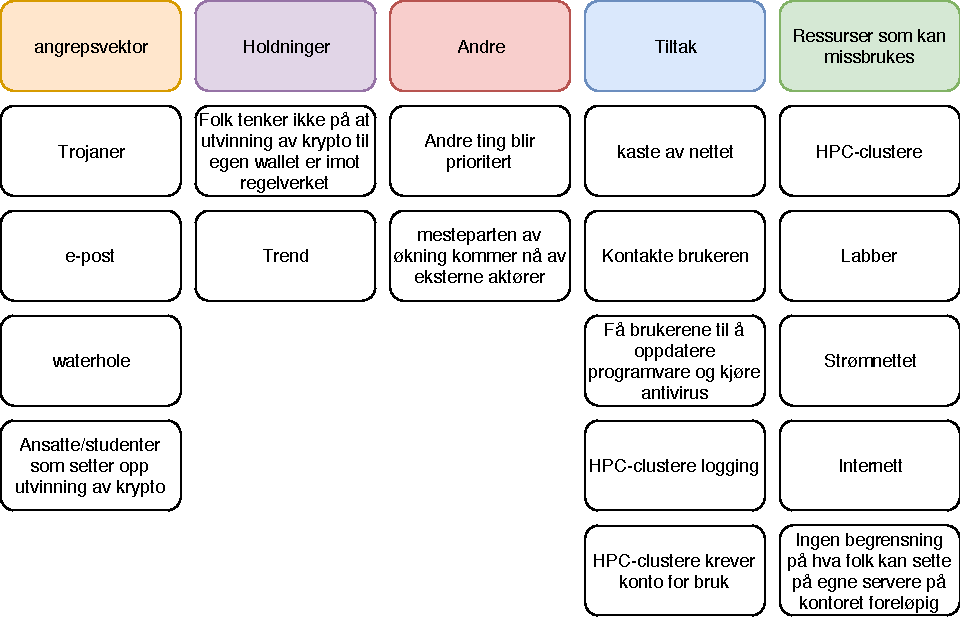
\includegraphics[scale=0.6]{case_3/bilder/AD.pdf}
    \label{fig:AD_miner}
    \caption[Analyse av intervju]{Hvordan fungerer utvinning av kryptovaluta ved NTNU?}
\end{figure}

Vi finner mulige årsaker og tiltak som er satt på plass, og forhåpentligvis er rotårsaken blant dem.


\subsection{Rotårsaksidentifisering}
\subsubsection{5 Whys}

\paragraph{Valg og ønsket utbytte av verktøy}
Ved å bruke 5 Whys ønsker  vi å finne ut hva som er rotårsaken til problemet. Målet her er å få frem så mange rotårsaker som mulig, som vi kan bruke på rotårsakselimineringen. 

\paragraph{Spesifiseringer}


\paragraph{Gjennomføring}
Med dette verktøyet tar vi utgangspunkt i casebeskrivelsen; nemlig rotårsaken til kryptoutvinning på NTNU. Ut fra dette brukte vi funnene fra analysen for å komme på årsaker, samt prøvde å idémyldre et par nye. For hver av disse årsakene ble det spurt: ``Hvorfor er dette en årsak av det originale problemet?''. For hvert svar spør vi hvorfor igjen og igjen helt til vi finner rotårsaken. Det ble tatt utgangspunkt i fem iterasjoner, men det er mulighet for flere eller færre avhengig av om spørsmålet kan besvares på en fornuftig måte. 


\subsubsection{Feiltreanalyse}
\paragraph{Valg og ønsket utbytte av verktøy}
Ved bruk av dette verktøyet ønsker vi å få en oversikt over koblinger mellom de forskjellige årsakene. Vi ønsker også å få sortert ut de årsakene som NTNU ikke har mulighet til å gjøre.

\paragraph{Spesifiseringer}


\paragraph{Gjennomføring}
Med dette verktøy tar vi utgangspunktet i resultatet fra 5 Whys til å finne rotårsakene. Her går vi steg for steg nedover og ser på hva som er årsaken til at enhver uønsket hendelse inntreffer.


\subsection{Rotårsakseliminering}
\subsubsection{Systematisk Innovativ Tenkning (SIT)}

\paragraph{Valg og ønsket utbytte av verktøy}
Ved å bruke SIT-metoden ønsker vi å få kreative idéer på hvordan vi kan finne en løsning til utvinning av kryptovaluta ved NTNU. 

\paragraph{Spesifiseringer}


\paragraph{Gjennomføring}
SIT burde helst gjennomføres av 10-12 personer, fra en rekke forskjellige fagområder, men siden vi ikke hadde så mange tok vi bare utgangspunkt i prosjektgruppen.


\subsection{Løsningsimplementering}
\subsubsection{Kraftfeltsanalyse}

\paragraph{Valg og ønsket utbytte av verktøy}
Ønsket utbytte fra kraftfeltsanalyse er å få vite hva som er for og hva som er imot implementering av tiltakene. Dette verktøyet gir en plan over hvilke tiltak som er lettest å gjennomføre.

\paragraph{Spesifiseringer}


\paragraph{Gjennomføring}
Kraftfeltsanalysen ble gjort ved at vi tok tiltakene fra problemelimineringen og hadde en idémyldring for å se hva som talte for tiltakene og hva som var imot. 

